\section{Opgaver}
\subsection*{Elektrostatik}
\begin{opgave}{Coulombkraften}
    To ladninger, $q_1$ og $q_2$ har en indbyrdes afstand $r$ til hinanden.
    \opg Bestem Coulombkraften fra den ene ladning på den anden i hvert af følgende tilfælde:
    \begin{enumerate}
        \item $r = \SI{1,00}{\metre}$, $q_1 = \SI{1,00}{\coulomb}$ og $q_2 = \SI{1,00}{\coulomb}$
        \item $r = \SI{1,00}{\metre}$, $q_1 = \SI{1,00}{\coulomb}$ og $q_2 = \SI{-1,00}{\coulomb}$
        \item $r = \SI{1,00}{\metre}$, $q_1 = \SI{1,00}{\coulomb}$ og $q_2 = \SI{2,00}{\coulomb}$
        \item $r = \SI{2,00}{\metre}$, $q_1 = \SI{1,00}{\coulomb}$ og $q_2 = \SI{1,00}{\coulomb}$
    \end{enumerate}
    \opg Beskriv med ord hvad der sker med Coulombkraften når den ene ladning skifter fortegn, dens størrelse fordobles og når ladningernes indbyrdes afstand fordobles.
    \opg Brug Newtons anden lov, ligning \eqref{mat:eq:N2}, til at bestemme accelerationen af hver ladning i tilfælde 1. Ladningernes masse er $m_1 = \SI{1,00}{\kilo\gram}$ og $m_2 = \SI{2,00}{\kilo\gram}$.
    \opg Bestem accelerationen af ladning 1 i tilfælde 2-4.
    \opg Beskriv med ord hvad der sker når ladningerne frigives i de fire tilfælde og sammenlign dem.
\end{opgave}

\begin{opgave}{Elektriske feltlinjer}
    Tegn de elektriske feltlinjer for følgende systemer:
    \opg To ladninger $+Q$ og $-2Q$.
    \opg To ladninger $+Q$ og $+2Q$.
    \opg Tre ladninger, $+Q$, som befinder sig på hjørnerne af en ligesidet trekant.
\end{opgave}

% \begin{opgave}{}
%     Skalare størrelser i fysik er bestemt kun med en talværdi, hvorimod vektorer har både en længde og en retning. Men typisk når vi taler om elektrisk strømstyrke har den også en retning. Hvordan tror du man vil kunne definere strømstyrke ud fra en vektor?
% \end{opgave}

\begin{opgave}{Tre ladninger på en linje}
    To punktladninger med ladning $+Q$ befinder sig ved positioner $x=-a$ og $x=a$.
    \opg Bestem kraften på en anden ladning $+q$ som funktion af dens position langs $x$-aksen.
    \opg Tegn en graf over kraften som funktion af position, og kommenter den generelle opførsel.
    \opg Hvordan vil ladningen bevæge sig når den er ved $x=0$?
    \opg For $x\gg a$, approksimer udtrykket for kraften. \textit{Hint: Hvad sker der hvis man lægger et lille tal til et stort tal?}
\end{opgave}

\begin{opgave}{Bohrs atommodel}
    Bohrs atommodel af hydrogenatomet består af en enkelt elektron, som kredser rund om en enkelt proton, i perfekte cirkulære baner. For at opretholde sådan en bane, skal der ifølge Newtons love være en indadgående centripetalkraft $F=mv^2/r$. Antag at elektronen befinder sig i en radius $r=\SI{0.53e-10}{\meter}$ (også kaldet en Bohr radius, $a_0$).
    \opg Hvad er størrelsen af Coulombkraften på elektronen? Dette kan gøres på en af to måder:
    \opg Med Newtonsk mekanik kan det vises at jævn cirkelbevægelse er opfyldt, hvis summen af alle kræfter er ovenstående centripetal kraft. Brug dette til at bestemme elektronens fart i cirkelbanen. \\[4mm]
    Jævn cirkelbevægelse betyder blandt andet at elektronen bevæger sig med samme fart hele tiden. Man kan bruge det til at argumentere for at elektronen kan beskrives med stedfunktionen
    \begin{align*}
        x(t) = vt + x_0,
    \end{align*}
    hvor $v$ er elektronens hastighed, $t$ er tiden og $x_0$ er stedet til tiden $t=0$. \\[4mm]
    Elektronens bane går igennem et område med areal $A$. Argumenter for at den mængde ladningen, der passerer igennem arealet er $q = -neAx(t)$, hvor $n$ er antalstætheden af ladning.
    \opg Estimer ud fra ovenstående strømstyrke en elektron ville generere i hydrogenatomet.
\end{opgave}

\begin{opgave}{Uendelig lang ladet linje}
    For at beregne det elektriske felt overalt i rummet fra en uendelig lang ladet linje med konstant ladningstæthed (ladning pr. afstand) $\lambda$ (med SI-enhed \si{\coulomb\per\meter}) bruges Gauss' lov. Det antages at linjen er i vakuum. En linje har cylindrisk symmetri, hvilket betyder at man kan dreje sit koordinatsystem omkring linjen uden at noget vil ændre sig. Det er derfor smart at bruge en cylinder med længden $L$ og radius $r$ som Gaussisk overflade.
    \opg Tegn situationen.
    \opg Vis at den mængde ladning, som er inden i cylinderen, der bruges som Gaussisk overflade er
    \begin{align*}
        Q_\mathrm{inde} = \lambda L.
    \end{align*}
    \opg Argumenter for at det elektriske felt peger direkte væk fra linjen overalt i rummet.
    \opg Cylinderen har to typer overflade: den krumme og endestykkerne. Udregn $\va E \cdot \dd{\va A}$ i begge tilfælde.
    \opg Det lukkede integral i Gauss' lov kan skrives som en sum af bidragene fra hver overflade. Lad $S_1$ angive den krumme overflade, og henholdsvis $S_2$ og $S_3$ angive de to endestykker. Løs integralet
    \begin{align*}
        \oint_S \va E \cdot \dd{\va A} = \int_{S_1} \va E \cdot \dd{\va A} + \int_{S_2} \va E \cdot \dd{\va A} + \int_{S_3} \va E \cdot \dd{\va A}.
    \end{align*}
    \opg Brug nu Gauss lov til at bestemme det elektriske felt overalt i rummet. \\
    \textit{Hint: Længden af cylinderen skulle gerne gå ud, så det endelige udtryk kun afhænger af $\lambda$, $r$ og nogle konstanter.}
\end{opgave}

\begin{opgave}{Uendeligt ladet plan}
    For at beregne det elektriske felt overalt i rummet fra en uendelig, homogen plan med konstant ladningstæthed (ladning per areal) $\sigma$ (med SI-enhed \si{\coulomb\per\meter\squared}) bruges Gauss' lov. Det antages at planen er i vakuum. Systemet er symmetrisk sådan at man kan spejle sit koordinatsystem i planen uden at noget vil ændre sig. Det er derfor smart at bruge en kvadratisk kasse med sidelængden $L$, hvor overfladen på hver side af planen er afstanden $r$ fra planen, som Gaussisk overflade.
    \opg Tegn situationen.
    \opg Vis at den mængde ladning, som er inden i kasse, der bruges som Gaussisk overflade, er
    \begin{align*}
        Q_\mathrm{inde} = \sigma L^2.
    \end{align*}
    \opg Argumenter for at det elektriske felt peger direkte væk fra planen overalt i rummet.
    \opg Kassen har to typer af overflade: dem som er parallelle med planen og dem, der er vinkelrette på den. Udregn $\va E \cdot \dd{\va A}$ i begge tilfælde.
    \opg Det lukkede integral i Gauss' lov kan skrives som en sum af bidragene fra hver overflade. Lad $S_i$ angive den $i$'te overflade. Løs integralet
    \begin{align*}
        \oint_S \va E \cdot \dd{\va A} = \sum_{i=1}^6 \int_{S_i} \va E \cdot \dd{\va A}.
    \end{align*}
    \opg Brug nu Gauss lov til at vise at det elektriske felt overalt i rummet er
    \begin{align*}
        \va E = \frac{\sigma}{2\epsilon_0}\vu n,
    \end{align*}
    hvor $\vu n$ er en normalvektor til planen.
    \opg Hvordan afhænger størrelsen af E-feltet af hvor i rummet man er?
\end{opgave}

\begin{opgave}{Ladet kugle I}
    En kugle med centrum i origo, $(0,0)$, placeres i vakuum og har den sfærisk symmetriske ladningstæthedsfordelingen
    %
    \begin{align*}
        \rho(r) = \begin{cases} \rho_0(R - r), \quad &r<R \\
        0, \qquad &r>R
        \end{cases} ,
    \end{align*}
    hvor $\rho_0$ og $R$ konstanter. Sfærisk symmetri betyder at $\rho$ kun afhænger af afstanden fra origo. Det er derfor smart at bruge en kugleskal med centrum i $(0,0,0)$, radius $r$ og tykkelse $\dd{r}$ som Gaussisk overfalde.
    \opg Hvad er radius af den ladede kugle?
    \opg Tegn kuglen og den Gaussiske overflade. \\[5mm]
    Nu vil vi gerne bestemme det elektriske felt indeni kuglen
    \opg For en kugleskal kan det vises at $\dd{V} = 4\pi r^2 \dd{r}$. Brug ligning \eqref{eq:volumenladning} til at vise den mængde ladning, som er indenfor kugleskallen, der bruges som Gaussisk overflade, er
    \begin{align*}
        Q_\mathrm{inde} = 4\pi\rho_0\left[\frac{1}{3}Rr^3 - \frac{1}{4}r^4 \right] \quad , \quad r<R.
    \end{align*}
    \opg Argumenter for at det elektriske felt peger direkte væk fra $(0,0)$ overalt i rummet.
    \opg Vis at
    %
    \begin{align*}
        \oint \va E \cdot \dd{\va A} = EA = 4\pi E r^2.
    \end{align*}
    %
    \opg Brug nu Gauss lov til at vise at det elektriske felt inde i kuglen er
    %
    \begin{align*}
        \va E = \frac{\rho_0r}{\epsilon_0}\left(\frac{1}{3}R - \frac{1}{4}r\right)\vu r \quad , \quad r<R,
    \end{align*}
    hvor $\vu r$ er en enhedsvektor, der peger væk fra origo.
    \opg Følg nu fremgangsmåden fra spørgsmål \textbf{2}-\textbf{6} og vis at
    %
    \begin{align*}
        \va E = \frac{\tilde{Q}}{4\pi \epsilon r^2}\vu r \quad , \quad r>R.
    \end{align*}
    %
    $\tilde{Q}$ er en konstant udtrykt ved de tidligere definerede parametre.
    \opg Hvilket kendt system svarer det til?
\end{opgave}

\begin{opgave}{Ladet kugle II}
    En ladet kugle med radius $R$ har en homogen ladningsfordeling $\rho=\rho_0=\text{konstant}$ for $r<R$ og $\rho=0$ for $r>R$, hvor $r$ er afstanden fra kuglens centrum. Kuglen antages at befinde sig i vakuum.
    \opg Hvad betyder det rent fysisk at $\rho(r>R) = 0$?
    \opg Brug Gauss' lov til at bestemme det elektriske felt $\va{E}$ for $r>R$.
    \opg Brug Gauss' lov til at bestemme det elektriske felt $\va{E}$ for $r<R$.
\end{opgave}

\begin{opgave}{Ladet cylinder}
    En uendelig lang cylinder med radius $a$ med ladningsfordelingen
    \begin{align*}
        \rho(r) = \begin{cases}
        \rho_0r/a \: , \quad r<a \\
        0 \: , \qquad r>a
        \end{cases} \: ,
    \end{align*}
    hvor $\rho_0=\text{konstant}$ og $r$ er afstanden fra centrum af cylinderen.
    \opg Brug Gauss' lov til at bestemme det elektriske felt $\va {E}$ i hele rummet.
    \textit{Hint: Se eksemplet i afsnit \ref{sec:gauss_lov_eksempel}.}
\end{opgave}

\begin{opgave}{Cylindrisk ladningsfordeling}
    En arbitrær kontinuert ladningsfordeling med total ladning $+Q$ er placeret i $yz$-planen med centrum i origo, og er rotationssymmetrisk om $x$-aksen. Derudover er en testladning $+q$ placeret et sted langs $x$-aksen. Vi vil gerne bestemme kraften på testladningen som funktion af $x$.
    \opg Betragt to ladninger $+Q/2$, hver især ved en position $y=\pm a$ langs $y$-aksen. Tegn situationen.
    \opg Hvad forventer du at kraften på ladningen $+q$ i de to tilfælde: $x=0$ og $x\gg a$? \textit{Hint: Hvor meget betyder en lille forskel i afstand, når to ting er langt væk fra hinanden?}
    \opg Brug Coulombs lov og superpositionsprincippet til at finde et udtryk for kraften som funktion af $x$.
    \opg Er dette som du forventer? Tegn en graf af $F(x)$ og vis at maksimum er når $x=a/\sqrt{2}$.
    \opg Betragt nu fire ladninger med $+Q/4$. To af dem er placeret på $y$-aksen ved $y=\pm a$, og de to andre på $z$-aksen ved $z=\pm a$. Bestem ligeledes kraften på ladningen $+q$ som funktion af $x$.
    \opg Nu ser vi på et stort antal, $N$, ladninger $+Q/N$, ligeligt fordelt på en cirkel med radius $a$ på $yz$-planet, og med centrum i origo. Hvad er kraften på ladningen $+q$ som funktion af $x$?
    \opg De forrige delopgaver refererer til en \emph{diskret} ladningsfordeling. Betragt nu en \emph{kontinuert} ladningsfordeling: En uendelig tynd ring af radius $a$, med total ladning $+Q$, placeret på $yz$-planet med centrum i origo. Brug dine svar fra de forrige opgaver til at gætte et udtryk for kraften på ladningen $+q$ som funktion af $x$. Brug derefter superpositionsprincippet og integraler til at vise eller afkræfte dit gæt.
    \opg En uendelig tynd, solid disk af radius $a$ og total ladning $+Q$ med ensartet ladningsfordeling er placeret på $yz$-planet med centrum i origo. Vis at kraften på ladningen $+q$ som funktion af $x$ er givet ved
    \[ F(x)=\frac{1}{4\pi\varepsilon_0}\frac{2Qq}{a^2}\left(1-\frac{x}{\sqrt{x^2+a^2}}\right). \]
\end{opgave}

\begin{opgave}{Ladede partikler i en trekant}
    Tre partikel med samme ladning er holdt stille så de danner en (vilkårlig!) trekant. Når der gives slip på partiklerne begynder de at bevæge sig i en lige linje. Vis at hvis dette skal kunne lade sig gøre, så må trekanten de danner til alle tider have samme vinkler som den originale trekant. Du kan antage at de er i vakuum og at ingen andre kræfter påvirker dem.
\end{opgave}

\subsection*{Magnetisme}
\begin{opgave}{Magnetisk felt}
    \opg Bestem det magnetiske felt fra ladningen i punktet $\va r = r \xhat$ i hvert af følgende tilfælde:
    \begin{enumerate}
        \item  $r = \SI{1,00}{\metre}$, $\va{v} = \SI{1,00}{\metre\per\second}\cdot\xhat$ og $q = \SI{1,00}{\coulomb}$
        \item $r = \SI{1,00}{\metre}$,  $\va{v} = \SI{1,00}{\metre\per\second}\cdot\yhat$ og $q = \SI{1,00}{\coulomb}$
        \item $r = \SI{1,00}{\metre}$,  $\va{v} = \SI{1,00}{\metre\per\second}\cdot\zhat$ og $q = \SI{1,00}{\coulomb}$
        \item $r = \SI{1,00}{\metre}$,  $\va{v} = \SI{1,00}{\metre\per\second}\cdot\yhat$ og $q = \SI{-1,00}{\coulomb}$
        \item $r = \SI{1,00}{\metre}$,  $\va{v} = \SI{1,00}{\metre\per\second}\cdot\yhat$ og $q = \SI{2,00}{\coulomb}$
        \item $r = \SI{1,00}{\metre}$,  $\va{v} = \SI{2,00}{\metre\per\second}\cdot\yhat$ og $q = \SI{1,00}{\coulomb}$
        \item $r = \SI{2,00}{\metre}$,  $\va{v} = \SI{1,00}{\metre\per\second}\cdot\yhat$ og $q = \SI{1,00}{\coulomb}$
    \end{enumerate}
    \opg Beskriv med ord hvad der sker med magnetfeltet når ladningen skifter fortegn, dens størrelse fordobles, dens bevægelsesretning ændres, dens hastighed fordobles og når ladningernes indbyrdes afstand fordobles.
    \opg Hvad er den magnetiske kraft på en ladning $Q = \SI{1,00}{\coulomb}$ i punktet $\va r = r \xhat$ med hastigheden $\va v' = \SI{1,00}{\metre\per\second}\cdot\zhat$ i hvert af tilfældende?
\end{opgave}

\begin{opgave}{Uniformt magnetfelt}
    I afsnit \ref{sec:uniformt_b-felt} blev kraften fra et uniformt magnetfelt på en punktladning i bevægelse beregnet.
    \opg Skitser situationen.
    \opg Forklar hvorfor ladningens position ikke blev betragtet i eksemplet.
    \opg Når tiden går ændres retningen på ladningens hastighed. Man kan vise ladningen kommer til at dreje rundt i en cirkel som tiden går. Forklar uden beregninger hvorfor dette sker.
    \opg Hvad ville der ske med ladningen, hvis den havde været påvirket af et uniformt elektrisk felt, $\va E = E_0 \zhat$, og ikke et magnetfelt.
\end{opgave}

\begin{opgave}{Amperes lov}
    Der er to vigtige argumenter i afsnit \ref{sec:lang_lige_leder} og alt kommer fra lederens symmetri og antagelsen om at den er uendelig lang. Forklar med egne ord argumenterne for at
    \opg magnetfeltet er cirkulært omkring lederen.
    \opg magnetfeltets størrelse kun afhænger af afstanden til lederen. \\[4mm]
    Hvis lederen ikke er uendelig lang er ovenstående analyse kun approksimativt sandt omkring midten af lederen.
    \opg Skitser det magnetisk felt for en endelig leder.
\end{opgave}

\begin{opgave}{To lange lige ledere}
    To uendeligt lange lige ledere med strømstyrkerne hhv. $\va I_1 = I_1 \xhat$ og $\va I_2 = I_2 \xhat$ placeres en afstand $d$ fra hinanden.
    \opg Skitser situationen.
    \opg Indtegn et koordinatsystem, hvor $x$-aksen placeres langs med den ene leder.
    \opg Bestem magnetfeltet fra den første leder på den anden.
    \opg Tiltrækkes de to ledere af hinanden eller frastøder de hinanden?
    \opg Hvad hvis strømmen går i hver sin retning af de to ledere?
    \opg Benyt superpositionsprincippet til at beregne magnetfeltet fra de to ledere i tilfældet hvor strømmene er parallelle i $xy$-planen.
\end{opgave}

\begin{opgave}{Forskellen på elektriske og magnetiske felter}
    En ladet partikel bevæger sig i et homogent felt.
    \opg Vis at partiklen altid bevæger sig i en parabel, hvis feltet er elektrisk.
    \opg Sammenlign ovenstående resultat med afsnit \ref{sec:uniformt_b-felt}.
    \opg Hvad ville der ske, hvis ladningen bevægede sig parallelt med et sådant magnetfelt?
\end{opgave}

% \begin{opgave}{}
%     Betragt en ring med total ladning $Q$, vis centrum ligger på $x$-aksen, og alle punkter på cirklen ligger en afstand $r$ fra origo. Linjen fra origo til ethvert punkt på cirklen danner en vinkel $\theta$ med $x$-aksen.
%     \opg Vis at det elektriske felt i origo er
%     \begin{equation}
%         \va{E}=-\frac{Q\cos\theta}{4\pi\varepsilon_0r^2} \xhat.
%     \end{equation}
%     Et dielektrikum med homogen polarisering $\va{P}=P\hat\va{x}$ indeholder et sfærisk hul med radius $r$, centreret i origo.
%     \opg Vis at overfladepolariseringsladningsdensiteten ved ethvert punkt på overfladen af hullet er $\rho_{sp}=-P\cos\theta$, hvor $\theta$ er vinklen mellem linjer fra origo til punktet, og $x$-aksen. Overvej nu et tyndt bånd på overfladen af hullet, hvor linjen der der forbinder origo til ethvert punkt på båndet danner vinklen $\theta$ med $x$-aksen.
%     \opg Vis at den totale ladning på båndet er
%     \begin{equation}
%         Q_\text{bånd}=-2\pi Pr^2\sin\theta\cos\theta\ \dd\theta.
%     \end{equation}
%     \opg Vis dermed at overfladepolariseringsladningen på overfladen af hullet danner et elektrisk felt i origo givet ved
%     \begin{equation}
%         \Delta\Vec{E}=\frac{P}{2\varepsilon_0}\int_0^\pi\sin\theta\cos^2\theta\ \dd\theta \ \xhat.
%     \end{equation}
%     \opg Anvend
%     \[ \int_0^\pi\sin\theta\cos^2\theta\ \dd\theta =\frac{2}{3} \]
%     til at vise at det elektriske felt i centrum af hullet er
%     \begin{equation}
%         \va{E}_\text{hul}=\Vec{E}_\text{diel}+\frac{\Vec{P}}{3\varepsilon_0},
%     \end{equation}
%     hvor $\Vec{E}_\text{diel}$ er det elektriske felt i dielektrikummet.
%     \opg Beregn forholdet mellem $\Vec{E}_\text{diel}$ og $\frac{\Vec{P}}{3\varepsilon_0}$ i glas ($\varepsilon_r=\SI{4.0}{}$).
% \end{opgave}

\begin{opgave}{Lang lige leder med udstrækning}
    I afsnit \ref{sec:lang_lige_leder} blev det magnetiske felt fra en uendelig tynd lang lige leder med strømstyrke $I$ bestemt. Situationen ændrer sig en smule, hvis lederen har en endelig tykkelse $R$, og strømstyrken uniformt fordelt over tværsnittet.
    \opg Argumenter for at udregningerne ikke ændrer sig i en afstand $r>R$, hvorfor magnetfeltet er det samme.
    \opg Argumenter for at integralet i Amperes lov er det samme indenfor og udenfor lederen:
    %
    \begin{align}
        \oint \va B \cdot \dd \va l = 2\pi B r,
    \end{align}
    %
    hvor $r$ er afstanden lederens centrum.
    \opg Vis at den indesluttede strøm i tilfældet $r<R$ er
    %
    \begin{align}
        I_\mathrm{inde} = I \frac{r^2}{R^2}.
    \end{align}
    %
    \opg Brug dette til at vise at
    %
    \begin{align}
        B = \begin{cases}
            \mu_0I/2\pi r, \quad &r>R \\
            \mu_0Ir/2\pi R^2, \quad &r<R
        \end{cases}
        .
    \end{align}
    %
    \opg Skitser funktionen $B(r)$.
    \opg Argumenter kvalitativt for hvordan funktionen $B(r)$ ville se ud hvis lederen var hul med en indre radius $R_0$ og skitser funktionen.
\end{opgave}

\begin{opgave}{Eleveksperiment}
    I et eksperiment har en elev målt strømstyrken gennem en LED over tid og har empirisk estimeret den til at følge funktionen $I=\left(\SI{0.06}{\ampere\second}\right)/\left(\SI{20}{\second}+t\right)$, hvor $t$ er tiden målt i sekunder (målingen starter ved $t=0$).
    \opg Brug at man i fysik godt betragte $\dd{t}$ som en variabel samt ligning \eqref{eq:current} til at vise at
    \begin{align*}
        \dd{q} = I\dd{t}.
    \end{align*}
    \opg Vis at ladningen, der er løbet gennem Amperemeteret i tidsrummet $t=0$ til $t=T$, er
    \begin{align*}
        q(t=T) - q(t=0) = \int_0^T I(t) \dd{t}.
    \end{align*}
    \opg Strømmen i kredsløbet tændes til tiden $t=0$. Hvad er $q(t=0)$?
    \opg Bestem den totale ladning, der har været gennem amperemeteret efter et minut.
\end{opgave}

\begin{figure}
    \centering
    \begin{subfigure}[t]{.47\textwidth}
        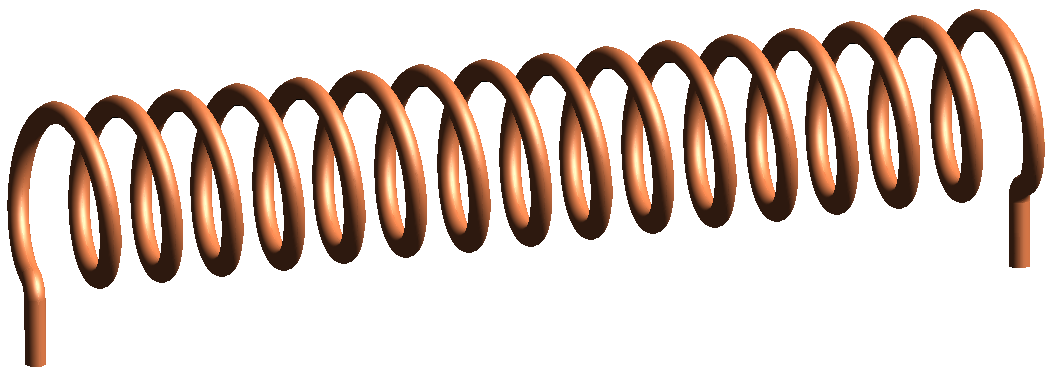
\includegraphics[width=\columnwidth]{opg/figurer/Solenoid-1.png}
        \caption{Illustration af en solenoide. Kilde: \cite{SolenoidWikipedia2019}}
        \label{fig:solenoide}
    \end{subfigure}
    %
    \hfill
    %
    \begin{subfigure}[t]{.47\textwidth}
        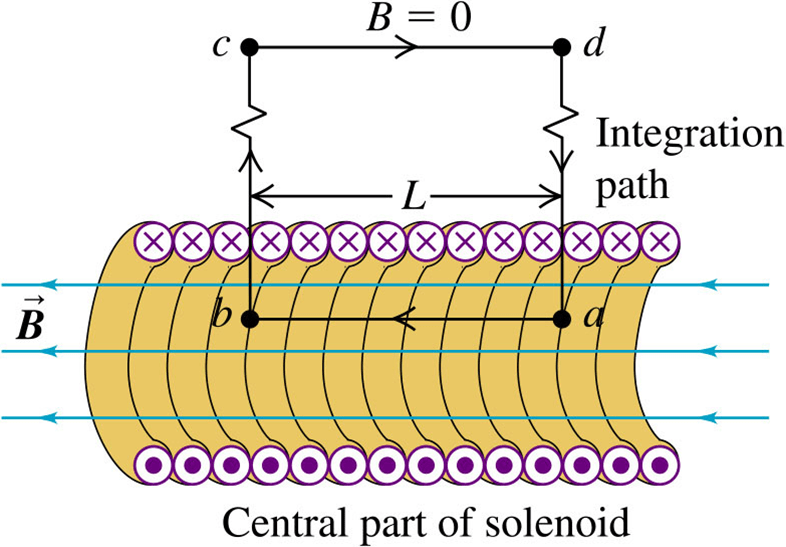
\includegraphics[width=\columnwidth]{opg/figurer/solenoid.png}
        \caption{Tegning af en solenoide med $n$ vindinger pr. længde, hvori der løber en strøm med strømstyrke $I$. Kilde: \cite{UY1ApplicationsAmpere2015}}
        \label{fig:solenoide_ampere}
    \end{subfigure}
    \caption{ }
\end{figure}
\begin{opgave}{Solenoiden}
    Afsnit \ref{sec:uniformt_b-felt} beskrev hvordan en ladning i et uniformt magnetfelt opfører sig. En måde at fremstille et (approksimativt) uniformt magnetfelt er ved brug af en solenoide, som illustreret i figur \ref{fig:solenoide}, hvori en strøm med strømstyrken $I$ løber. Det antages at solenoiden befinder sig i vakuum, at den er meget lang, og at antallet af  vindinger pr. længde, $n$, er så stor at solenoiden kan beskrives som ringe af strøm, der ligger helt tæt op ad hinanden. Der vælges en Ampereløkke, som den i figur \ref{fig:solenoide_ampere}, hvor punkterne $a$ og $b$ placeres midt i solenoiden og punkterne $c$ og $d$ placeres uendeligt langt væk fra solenoiden. Bredden af løkken kaldes $L$ og hele løkken er placeret ved midten af solenoiden.
    \opg Brug højrehåndsreglen til at bestemme retningen på det magnetiske felt midt i solenoiden.
    \opg På baggrund af antagelserne er størrelsen af det magnetiske felt på hele linjestykket $cd$ 0. Forklar hvorfor det er tilfældet.
    \opg Argumenter for at magnetfeltet udenfor solenoiden omkring Ampereløkken er parallelt med feltet indeni solenoiden.
    \opg Brug ovenstående argumenter til at vise at
    \begin{align*}
        \oint_P \va B \cdot \dd{\va l} = BL.
    \end{align*}
    \opg Vis at den indesluttede strøm er
    \begin{align*}
        I_\mathrm{inde} = nLI.
    \end{align*}
    \opg Brug Amperes lov til at vise at magnetfeltet inde i midten af solenoiden er
    \begin{align} \label{eq:b_solenoide}
        B = \mu_0nI.
    \end{align}
    \opg Argumenter, ud fra antagelserne, for at magnetfeltet er uniformt omkring midten af solenoiden med feltstyrken givet i ligning \ref{eq:b_solenoide}.
\end{opgave}

\subsection*{Induktion}
\begin{figure}
    \centering
    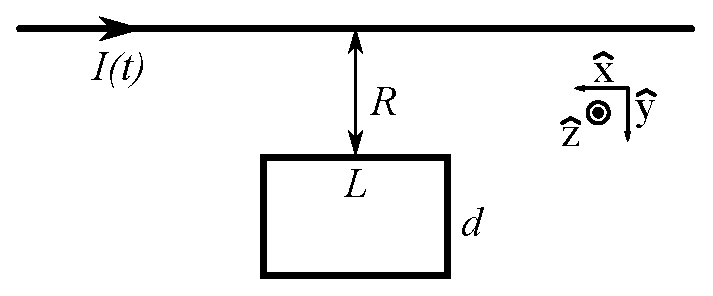
\includegraphics[width=.6\columnwidth]{opg/figurer/induktion.eps}
    \caption{En rektangulær løkke placeret i forhold til en lang lige leder med tidsafhængig strømstyrke.}
    \label{fig:induktion}
\end{figure}
\begin{opgave}{Induktion I}
    En rektangulær løkke af størrelsen $L\times d$ placeres i en afstand $R$ fra en lang lige leder med strømstyrken\footnote{Vekselstrøm kan beskrives med en strømstyrke på denne måde.} $I(t) = I_0\cos(\omega t)$ således at den fjerne del af rektanglen er i afstanden $R+d$ fra fra den lange lige leder -- se figur \ref{fig:induktion}. Induktionen sker i løkken, hvorfor man skal integrere over den overflade løkken udspænder.
    \opg Skraver det område man integrere over i figuren.
    \opg Argumenter for at magnetfeltet i $xy$-planen er uafhængigt af $x$- og $z$-koordinatet, $\va B = \va B(t,y)$.
    \opg Vis at fluxen gennem rektanglen er
    %
    \begin{align}
        \Phi_B = \int_R^{R+d} \int_0^L \va B \cdot \zhat \dd{x}\dd{y} = -\frac{\mu_0LI(t)}{2\pi}\ln\left(\frac{R+d}{R}\right).
    \end{align}
    \opg Vis ved brug af Faradays lov at
    %
    \begin{align}
        \mathcal{E} = \frac{\mu_0LI_0\omega}{2\pi}\ln\left(\frac{R}{R+d}\right)\sin(\omega t).
    \end{align}
    %
    \opg Forklar ud fra Lenz’ lov hvordan strømmen løber i løkken som tiden går.
    \opg En elpære med effekt $P$ tilsluttes løkken. Brug at $P=VI$ til at vise at strømstyrken igennem pæren er
    %
    \begin{align}
        I = \frac{P}{\mathcal{E}} = \frac{2\pi P}{\mu_0LI_0\sin(\omega t)\ln\big[R/(R+d)\big]}.
    \end{align}
\end{opgave}

\begin{figure}
    \centering
    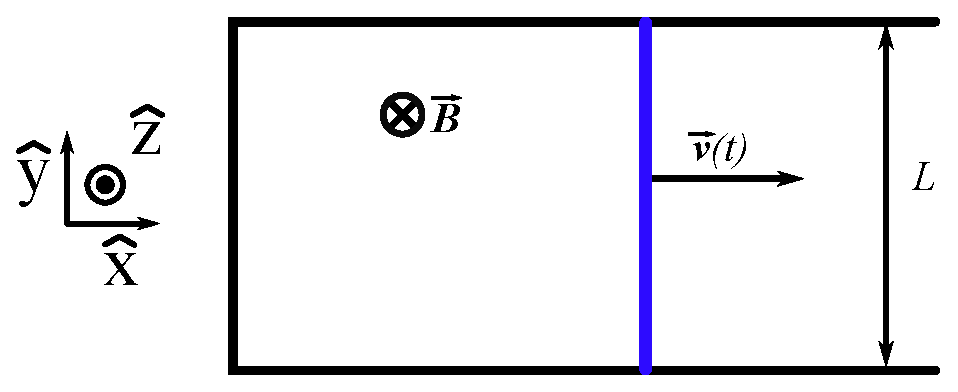
\includegraphics[width=.65\columnwidth]{opg/figurer/induktion_ii.eps}
    \caption{En lineær leder glider vinkelret og friktionsløst med hastighed $v(t)$ på en åben rektangulær leder.}
    \label{fig:induktion_ii}
\end{figure}
\begin{opgave}{Induktion II}
    En lineær leder glider vinkelret og friktionsløst med hastigheden
    %
    \begin{align} \label{eq:fart_induktion}
        \va v(t) = \Big(at + v_0\Big)\xhat
    \end{align}
    %
    på en åben rektangulær leder med bredden $L$, se figur \ref{fig:induktion_ii}. Man kan vise at stedfunktionen for den lineære leder er
    %
    \begin{align} \label{eq:sted_induktion}
        \va r(t) = x(t)\xhat = \left[\frac{1}{2}at^2 + v_0t + x_0\right]\xhat.
    \end{align}
    %
    Opsætningen placeres i et konstant uniformt magnetfelt vinkelret på opstillingen med styrken $\va B(t) = -B_0 \zhat$
    \opg Vis at stedfunktionen \ref{eq:sted_induktion} opfylder at hastighedsfunktionen er ligning \ref{eq:fart_induktion} ud fra definitionen på fart, ligning \ref{mat:eq:hast}.
    \opg Argumenter for at arealelementet i ligning \ref{eq:magnetisk_flux} er
    %
    \begin{align}
        \dd{\va A} = \zhat \dd{x}\dd{y}.
    \end{align}
    %
    \opg Forklar at koordinaterne for hjørnerne i den lukkede rektangel er $(0,0),(0,L),(x(t),L),(x(t),0)$.
    \opg Argumenter for at fluxen er givet ved integralet
    %
    \begin{align}
        \Phi_B = \int_0^L \int_0^{x(t)} \va B \cdot \zhat \dd{x'}\dd{y}.
    \end{align}
    %
    \opg Løs integralet for at vise at
    %
    \begin{align}
        \Phi_B = -B_0L\left[\frac{1}{2}at^2 + v_0t + x_0\right].
    \end{align}
    %
    \opg Vis at den elektromotoriske kraft i kredsløbet er
    %
    \begin{align}
        \mathcal{E} = B_0L\Big[at + v_0\Big].
    \end{align}
    %
    \opg Nu kobles en elpære, der bruger effekten $P$ til kredsløbet. Brug at sammenhængen mellem modstanden, strømstyrke og spændingsforskel er $V^2=PR$ til at vise at modstanden, $R$, i pæren er
    %
    \begin{align} \label{eq:induktion_ii_modstand}
        R(t) = \frac{(B_0L)^2}{P}\Big[at + v_0\Big]^2.
    \end{align}
    %
    \opg Hvilken type funktion er $R(t)$?
    \opg Skitser spændingen som funktion af tid. \\
    \textit{Hint: Det vigtige er hvad der sker over tid, så lad være med at bekymre dig om at tegne funktionen for nogle bestemte værdier af konstanterne.}
    \opg Hvad er modstanden i en $\SI{40}{\watt}$-pære til tiden $t = \SI{0}{\second}$, hvis $B_0 = \SI{1,2}{\tesla}$, $L = \SI{1,5}{\metre}$ og $v_0 = \SI{50}{\kilo\metre\per\hour}$?
\end{opgave}